\documentclass[11pt, oneside]{article} 
\usepackage{geometry}
\geometry{letterpaper} 
\usepackage{graphicx}
	
\usepackage{amssymb}
\usepackage{amsmath}
\usepackage{parskip}
\usepackage{color}
\usepackage{hyperref}

\graphicspath{{/Users/telliott_admin/Tex/png/}}
% \begin{center} 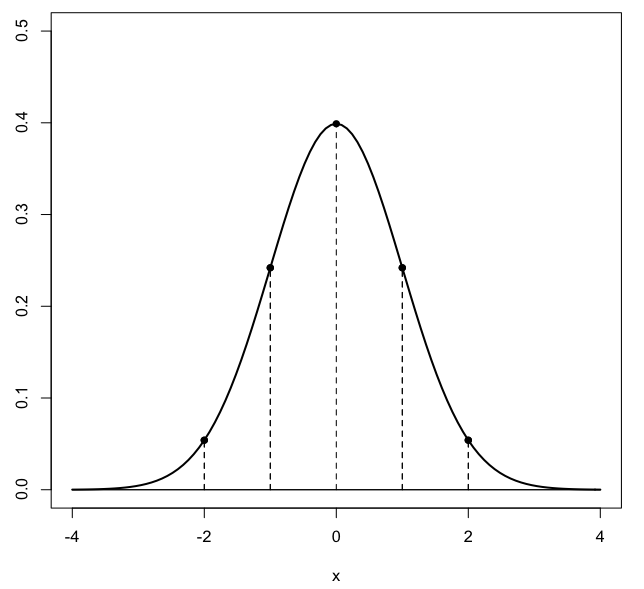
\includegraphics [scale=0.4] {gauss3.png} \end{center}

%break
\title{Techniques}
\date{}

\begin{document}
\maketitle
\Large

\label{sec:Techniques_of_integration}

This chapter surveys some useful techniques for integration.  There are four approaches commonly given in introductory calculus:

$\bullet$ $u$ substitution

$\bullet$ trigonometric substitution

$\bullet$ integration by parts (IBP)

$\bullet$ partial fractions

We'll take a quick look at all of these.  

Here is an example for substitution.  
\[ \int \tan t \ dt \]
No doubt, when students first see this, they are mystified.  Have I ever seen any $f(x)$ that gives the tangent as its derivative?

Insight comes from writing the two parts of the tangent:
\[ \int \frac{\sin t}{\cos t} \ dt \]
We recognize that 
\[ \frac{d}{dt} \cos t = - \sin t  \]
Let
\[ u = \cos t \]
\[ du = - \sin t \ dt \]
the integral is
\[ - \int \frac{1}{u} \ du = - \ln u \]
\[ = - \ln \cos t \]
Since the cosine can take on values where the logarithm is not defined (i.e. $< 0$) the answer is usually given as
\[ = - \ln |\cos t| \]

Another classic one is the secant
\[ \int \sec x \ dx \]
There is also a trick to this one, multiply top and bottom by $\sec x + \tan x$
\[ \int \sec x \ \frac{\sec x + \tan x}{\sec x + \tan x} dx \]
You see that $\sec^2 x$ is the derivative of $\tan x$ and $\sec x \tan x$ is the derivative of $\sec x$ so this is just
\[  \int \frac{1}{u} \ du  \]
again, namely
\[ \int \sec x \ dx = \ln | \sec x +  \tan x \ | + C \]

Now compare these two integrals
\[ \int x \ \sqrt{1-x^2}  \ dx \]
\[ \int \sqrt{1-x^2} \ \ dx \]

The extra value of $x$ makes a big difference in the first one.  I look at the $x$ and know we have the derivative of what is inside the square root.  So let $u = 1-x^2$ and then $du = -2x \ dx$ and the integral becomes
\[ \int (- \frac{1}{2}) \ \sqrt{u} \ du = - \frac{1}{3} u^{3/2} \]
\[ =  - \frac{1}{3} (1-x^2)^{3/2} \]

This integral comes up in the problem of finding the average value of $x$ over the unit circle (or half-circle).  Since it's an even function of $x$, the result is zero, if the bounds are centered around zero like as $[-b,b]$.

With practice you will not need to write the substitution.  Just say, OK, I know I have the $x$.  Now the integral of the square root is $(1-x^2)^{3/2}$.  I need one factor of $2/3$ to neutralize the exponent, and another factor of $-1/2$ for $-x^2$ so I write the answer, and then check by differentiating.

For the second integral, we do not have the derivative of what's inside the square root.
\[ \int \sqrt{1-x^2} \ \ dx \]
Nevertheless, this one can be solved using what is called a trig substitution.  Consider this figure
\begin{center} 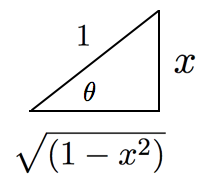
\includegraphics [scale=0.5] {trig1.png} \end{center}

We draw a generic right triangle.  The figure labels that angle as $\theta$ (I often use $t$ just because it's easier to type).  Since we have $\sqrt{1-x^2}$, we know we will need $x$ for the side opposite the angle and $1$ for the hypotenuse.  So let

\[ x = \sin \theta \]
\[ dx = \cos \theta \ d \theta \]
And from Pythagoras
\[ \sqrt{1-x^2} = \cos \theta \]

Take a look at
\[ \int \sqrt{1-x^2} \ dx \]
The square root is on the top.  If it were on the bottom, the cosines would cancel (we will see that problem later).  We get
\[ \int \cos^2 \theta \ d \theta \]

This is an integral that comes up a lot, and there are several ways to do it.  We will solve this \hyperref[sec:Cosine_squared]{\textbf{soon}}.

For now, the answer is:
\[ \int \cos^2 \theta \ d \theta = \frac{1}{2} \ [ \ \theta + \sin \theta \cos \theta \ ] \]

This is easily verified by differentiating:
\[ \cos^2 \theta = \frac{1}{2} \  [ \ 1 - \sin^2 \theta + \cos^2 \theta \ ] \]
\[ = \frac{1}{2} \ [ \ \cos^2 \theta + \cos^2 \theta \ ] \]

Although people always do this problem as described, it's worth pointing out that we could do a different trigonometric substitution.  There is no reason not to write

\[ x = \cos \theta \]
\[ dx = - \sin \theta \ d \theta \]
\[ \sqrt{1 - x^2} = \sin \theta \]
and so
\[ \int \sqrt{1 - x^2} \ dx = - \int \sin^2 \theta \ d \theta \]

Again, the answer is:
\[ \int \sin^2 \theta \ d \theta = \frac{1}{2} \ [ \ \theta - \sin \theta \cos \theta \ ] \]

Of course this is true since
\[ \sin^2 \theta + \cos^2 \theta = 1 \]
\[ \int \sin^2 \theta \ d \theta + \int \cos^2 \theta \ d \theta = \int 1 \ d \theta = \theta  \]

If you add the two answers given for $\sin^2$ and $\cos^2$ you'll get the same result.

\subsection*{change of variables}

$u$-substitution and trigonometric substitution, or just substitution in general, has one subtle aspect, which is that if you change the variable, you must also change the bounds.  Either that, or change back to the original variable at the end.  For example, above we had

\[ \int x \ \sqrt{1-x^2}  \ dx \]
We let $u = 1-x^2$ and then $du = -2x \ dx$ and the integral becomes
\[ \int (- \frac{1}{2}) \ \sqrt{u} \ du = - \frac{1}{3} u^{3/2} \]
Suppose the bounds on $x$ were $[0,1]$
\[ \int_0^1 x \ \sqrt{1-x^2}  \ dx \]
The bounds on the integral in $u$ must be adjusted:
\[ x = 0, \ \ \ \ u = 1 \]
\[ x = 1, \ \ \ \ u = 0 \]
so
\[ - \frac{1}{3} u^{3/2} \ \bigg |_1^0 = \frac{1}{3} u^{3/2} \ \bigg |_0^1 = \frac{1}{3} \]
Alternatively, switch back to $x$
\[  - \frac{1}{3} u^{3/2} = - \frac{1}{3} (1-x^2)^{3/2} \ \bigg |_0^1 \]
\[ = - \frac{1}{3} (0 - 1) = \frac{1}{3} \]

Our second example above was
\[ \int \sqrt{1 - x^2} \ dx = \frac{1}{2} \ [ \ \theta + \sin \theta \cos \theta \ ] \]
Suppose the bounds on $x$ were $[0,1]$.  The first substitution we tried was 
\[ x = \sin \theta \]
To find the bounds on $\theta$, we must ask, what value of $\theta$ gives the correspond value of $x$?  We obtain
\[ x = \sin \theta = 0, \ \ \ \  \theta = 0 \]
\[ x = \sin \theta = 1, \ \ \ \  \theta = \pi/2 \]
So
\[  \frac{1}{2} \ [ \ \theta + \sin \theta \cos \theta \ ] \ \bigg |_0^{\pi/2} \]
The second term is $0$ at both bounds, and the first is $\pi/2$, which is our answer.

Alternatively, we can switch the variable back to $x$
\[ x = \sin \theta \]
\[ \theta = \sin^{-1} x \]
so the answer is
\[  \frac{1}{2} \ [ \ \theta + \sin \theta \cos \theta \ ]  \ \bigg |_0^{\pi/2} = \frac{1}{2} \ [ \ \sin^{-1} x + x \sqrt{1-x^2} \ ]  \ \bigg |_0^{1} \] 
And again, the second term is zero at both bounds.  The first term is just $\pi/2$, which is the same as we obtained before.

\section*{integration by parts (IBP)}

Another approach to the integral uses integration by parts.

IBP is a reversal of the product rule.  Consider two functions of $x$, $u(x)$ and $v(x)$.  (Drop the $(x)$ notation for the moment).

\[ (uv)' = v \ du +  u \ dv \]
The idea is that when we integrate this we will have
\[ \int (uv)' = uv = \int v \ du +  \int u \ dv  \]
Rearranging, we obtain
\[ \int u \ dv = uv - \int v \ du  \]
Just to be clear, with an explicit independent variable $x$ this is:
\[ \int u \frac{dv}{dx} \ dx = uv - \int v \frac{du}{dx} \ dx \]
Here is a figure from Strang:
\begin{center} 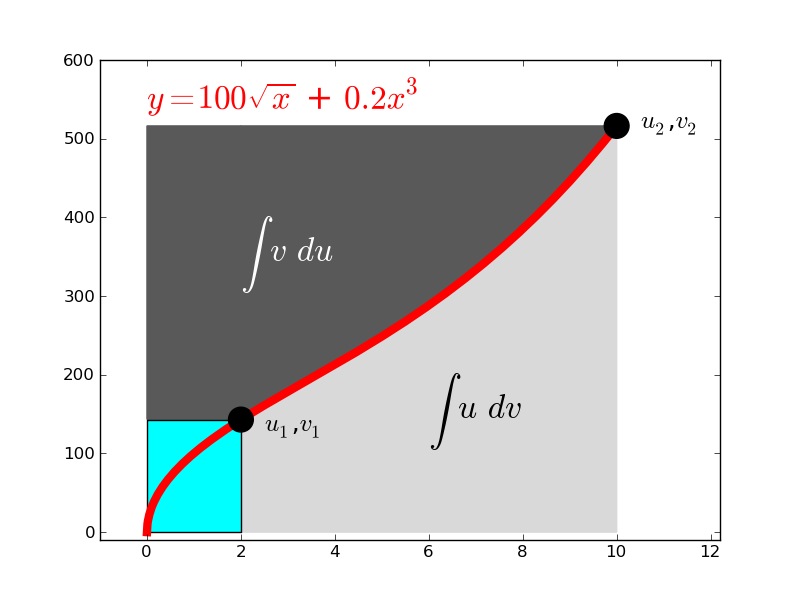
\includegraphics [scale=0.5] {ibp.png} \end{center}

\subsection*{examples}
As a first example, take 
\[ \int x \ e^x \ dx \]
If this were
\[ \int x \ e^{x^2} \ dx \]
there would be no problem, because upon differentiating $x^2$ using the chain rule, we will get the $x$ that we see in the example.  For the first problem, write
\[ u = x \]
\[ du = dx \]
\[ dv = e^x \ dx \]
this is what we have.  Now let's see how this simplifies things
\[ v = \int e^x \ dx = e^x \]
Using the formula
\[ \int u \ dv = uv - \int v \ du \]
\[ uv = xe^{x} \]
\[ \int v \ du = \int e^{x} \ dx = e^{x} \]
So
\[ \int x e^x \ dx =  xe^{x} - e^{x} \]

Check
\[ \frac{d}{dx} \ [ \ xe^{x} - e^{x}\ ]  = xe^{x}  \]
It is clear that the extra term in the answer is there to eliminate an extra term in the derivative.  This pattern is generally true with integration by parts.

The problem we had above, $\cos^2 x$, can be solved by this method.  But let's wait and give it its own section.

\subsection*{exponential}
Consider the question:  what is the average value of $x$ for the negative exponential function over the interval $[0,\infty)$?

Start with 
\[ \int_0^{\infty} \ e^{-kx} \ dx \]
\[ = -\frac{1}{k} e^{-kx} \ \bigg |_0^{\infty}    \]

Here we are faced with the problem of evaluating a function at the point $x = \infty$ but \emph{infinity is not a number}.  The approach is to evaluate the expression at some very large bound $b$, and then ask what happens if $b \rightarrow \infty$.  (See \hyperref[sec:Improper_integrals]{\textbf{here}}).
  
At the upper bound we get zero, and at the lower bound we are subtracting $-1/k$ so
\[ \int_0^{\infty} \ e^{-kx} \ dx = \frac{1}{k} \]

Now we want
\[ \int_0^{\infty} x \ e^{-kx} \ dx \]
Let 
\[ u = x \]
\[ du = dx \]
\[ dv =  e^{-kx} \ dx \]
\[ v = -\frac{1}{k} e^{-kx} \]

So IBP says
\[ \int u \ dv = uv - \int v \ du \]
\[ \int x \ e^{-kx} \ dx = -\frac{x}{k} e^{-kx} + \int \frac{1}{k} \ e^{-kx} \ dx \]
\[ = \ [ \ -\frac{x}{k} e^{-kx} - \frac{1}{k^2} \ e^{-kx} \ ] \ \bigg |_0^{\infty}  \]

At the lower limit the first term is zero and the second $-1/k^2$ which we change to $1/k^2$ by subtraction.  At the upper limit, the second term is a negative exponential so that goes to zero as $x \rightarrow \infty$.  

The first term is more complicated.  
\[ \lim_{x \rightarrow \infty} \ x e^{-kx} = \ ? \]
Rewrite it as a ratio:
\[ = \lim_{x \rightarrow \infty} \ \frac{x}{e^{kx}}  \]
We get infinity for both top and bottom and so invoke \hyperref[sec:Hopital]{\textbf{L'Hospital}}:
\[ = \lim_{x \rightarrow \infty} \ \frac{1}{ke^{kx}} = 0 \]
The final answer here is
\[ \int_0^{\infty} x \ e^{-kx} \ dx = \frac{1}{k^2}  \]

In fact, we can solve this integral for any power $x^n$ in the numerator.  Just invoke L'Hospital $n$ times. We will see this elsewhere (\hyperref[sec:Exponential_distribution]{\textbf{here}}).

By now, you should have a good handle on the integral as a measure of the area between the curve $f(x)$ and the $x$-axis.

\subsection*{below the x-axis}

One question we haven't dealt with is what happens when the curve dips below the $x$-axis.  Consider the line $y = x - 1$ which crosses the $x$-axis at $x = 1$ and the $y$-axis at $y = -1$.

\[ \int_0^1 x - 1 \ dx = \frac{x^2}{2} - x \ \bigg |_0^1 \]
\[ = \frac{1}{2} - 1 = - \frac{1}{2} \]

The absolute value of the area is correct but the sign is negative.  When we integrate a function that dips below the $x$-axis, the result will be negative.

\begin{center} 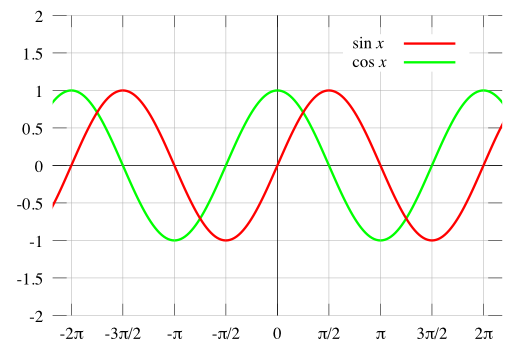
\includegraphics [scale=0.4] {sine_cosine_wikipedia.png} \end{center}

A further demonstration of this is the trigonometric functions $\sin x$ and $\cos x$:

They apparently spend as much of the time below the $x$-axis as above it.  These functions repeat with a period of $2 \pi$.  A consequence of this is that the integral of sine or cosine over a period of exactly $2 \pi$ is always equal to zero, regardless of the exact starting point.

\[ \int_0^{2\pi} \sin x \ dx = - \cos x \ \bigg |_0^{2\pi} = - (-1) - 1 = 0 \]

This is true for \emph{any} bounds whose difference is $2 \pi$.

\subsection*{area between two curves}
A common application of integrals is to give the area between two curves, which may be obtained simply by subtracting one function from another and integrating the difference.

\[ A = \int f(x) - g(x) \ dx \]

\subsection*{an easy problem}
Consider the two curves $y = \sqrt{x}$ and $y = x^2$.  These curves cross at
\[ \sqrt{x} = x^2 \]
We can see by inspection that this happens at $x = 0$ and $x = 1$.

In this region ($0 \le x \le 1$) the square root is larger than the square.

Furthermore, we already calculated that the part below $y = x^2$ is $1/3$ of the area of the rectangle with corners $(0,0)$ and $(x,y)$.  The same is true for the area above the square root.  From this we can predict what the result will be.

\[ A = \int f(x) - g(x) \ dx \]
For this problem
\[ A = \int_0^1 \sqrt{x} - x^2 \ dx \]
\[ = \frac{2}{3} x^{3/2} - \frac{x^3}{3} \ \bigg |_0^1  \]
\[ = \frac{2}{3} - \frac{1}{3} = \frac{1}{3} \]

\subsection*{a problem done two ways}
Consider $y = \ln x$.  This can be done two ways, as the figure shows.  We can use $x$ as the variable or $y$.
\begin{center} 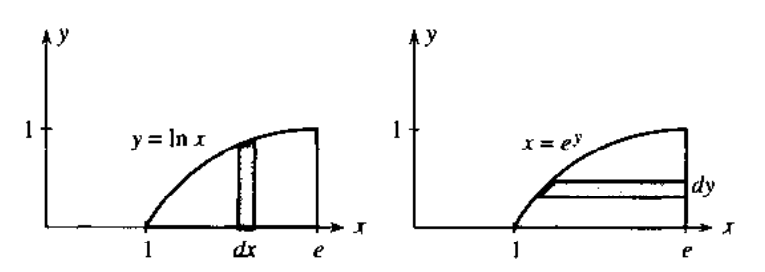
\includegraphics [scale=0.4] {log_plot.png} \end{center}

The standard approach would be $x$.  We want
\[ \int_1^e \ln x \ dx \]

We recall fooling around with the derivatives of products to pull this up:
\[ = x \ln x - x \ \bigg |_1^e \]
\[ = \ [ \ e - e \ ] \ - \ [ \ 0 - 1 \ ] \ = 1 \]

It's the other way that we subtract $f(x) - g(x)$:

\[ = \int (e - e^y) \ dy \]
\[ = ey - e^y \ \bigg |_0^1 \]
\[ = \ [ \ e - e^1 \ ] - \ [ \ 0 - 1 \ ] \]
\[ = 1 \]

That looks very smooth but it's got a lot of calculus in it!

\subsection*{a more complicated problem}

Consider the two curves $y = x$ and the unit circle $y = \sqrt{1 - x^2}$.
\begin{center} 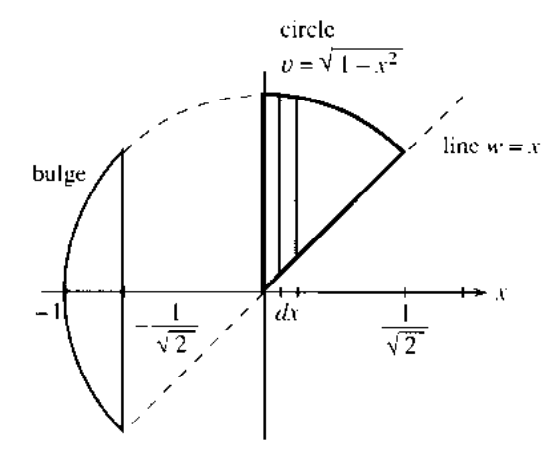
\includegraphics [scale=0.4] {between_curves.png} \end{center}
We see that the circle lies above the line for most of its length.  However, it's complicated.  Part of the figure is below the $x$-axis, and there is a bulge on the left end.

The key is that we must appreciate the relationship (know which is on top) in order to do integrals of differences between curves properly.

First solve for the points where the two curves cross:
\[ y = x = \sqrt{1 - x^2} \]
\[ 2x^2 = 1 \]
\[ x = \pm \sqrt{1/2}\ = \pm \frac{1}{\sqrt{2}} \]
\[ y = \pm \frac{1}{\sqrt{2}} \]

The area of the sector in the first quadrant is pretty easy.
\[ A = \int_0^{1/\sqrt{2}} \sqrt{1 - x^2}  - x \ dx \]
\begin{center} 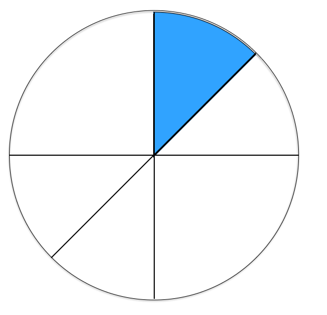
\includegraphics [scale=0.4] {between_curves2.png} \end{center}

We referred to the solution of $\int \sqrt{1 - x^2} \ dx$ previously in this chapter, and we will actually finally solve it in the next.  For now, just assume the result:

\[ = \frac{1}{2} \ [ \ \sin^{-1} x + x \sqrt{1-x^2} \ ] \ - \frac{x^2}{2} \ \bigg |_0^{1/ \sqrt{2}} \]
At the lower bound everything including $\sin^{-1} x$ is zero, and at the upper bound we have
\[ =  \frac{1}{2} \ [ \ \frac{\pi}{4} + \frac{1}{\sqrt{2}} \ \frac{1}{\sqrt{2}} \ ] - \frac{1}{4} = \frac{\pi}{8} \]
which we confirm from elementary geometry is just a slice of the pie.

For the area to the left of the $y$-axis we must think a little more.  The line $y=x$ dips below the $x$-axis, so the integral of the second part $g(x)$
\[ \int_{-1/\sqrt{2}}^0 x \ dx \]
is negative.

It's probably less confusing to just do the parts above and below the $x$-axis separately!

\begin{center} 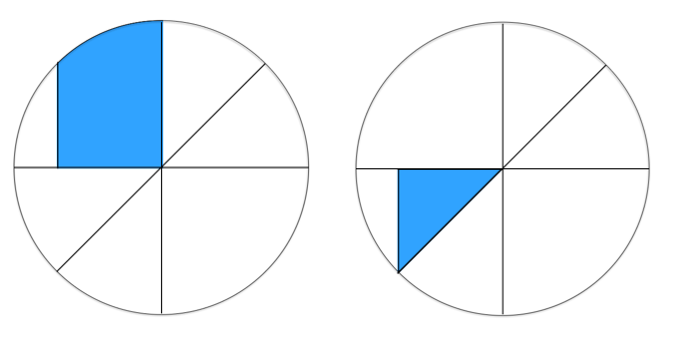
\includegraphics [scale=0.4] {between_curves3.png} \end{center}

The area above the $x$-axis is
\[ A = \frac{1}{2} \ [ \ \sin^{-1} x + x \sqrt{1-x^2} \ ] \ \bigg |_{-1/ \sqrt{2}}^0 \]
At the upper bound, we have again zero, and at the lower bound
\[ \frac{1}{2} \ [ \ - \frac{\pi}{4} + (-\frac{1}{\sqrt{2}}) \ \frac{1}{\sqrt{2}} \ ] \]
which must be subtracted, so we change signs and obtain
\[ \frac{\pi}{8} + \frac{1}{4} \]
This corresponds to a slice of the pie plus the triangle beneath it, which has two sides of length $1/\sqrt{2}$ and area $1/4$.

For the area below the $x$-axis:
\[ \int_{-1/ \sqrt{2}}^0 x \ dx \]
\[ = \frac{x^2}{2} \ \bigg |_{-1/ \sqrt{2}}^0 = - \frac{1}{4} \]
The area below the $x$-axis is \emph{minus} the result of the integral (the integral yields a negative area).

So lose the minus sign
\[ A = \frac{1}{4} \]

The total for this region (between $- 1/\sqrt{2}$ and $0$) is then just
\[ \frac{\pi}{8} + \frac{1}{4} + \frac{1}{4} = \frac{\pi}{8} + \frac{1}{2} \]
This is effectively a slice of pie plus a triangle of base $2/\sqrt{2}$ and height $1/\sqrt{2}$.

\begin{center} 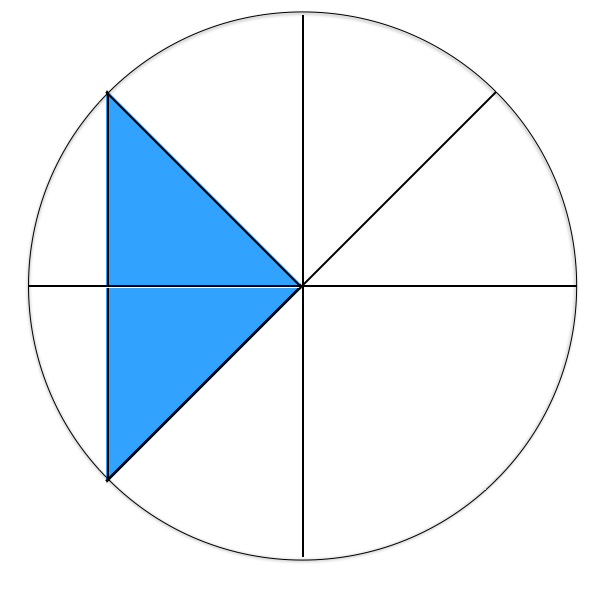
\includegraphics [scale=0.23] {between_curves5.png} \end{center}

The third part is the bulge to the left of $x = - 1/\sqrt{2}$.  

\begin{center} 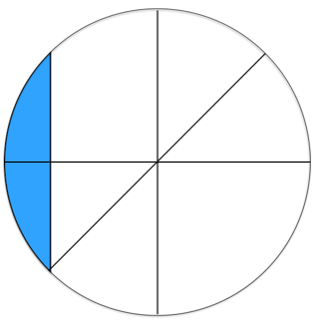
\includegraphics [scale=0.4] {between_curves4.png} \end{center}

We will calculate the area above the $x$-axis and multiply by two:
\[ A = 2 \int_{-1}^{-1/\sqrt{2}} \sqrt{1 - x^2} \ dx \]
\[ = 2 \ \frac{1}{2} \ [ \ \sin^{-1} x + x \sqrt{1-x^2} \ ]  \ \bigg |_{-1}^{-1/ \sqrt{2}} \]
The leading factors cancel.
\[ =  \sin^{-1} x + x \sqrt{1-x^2} \ ]  \ \bigg |_{-1}^{-1/ \sqrt{2}} \]

At the upper bound we have (as we found before)
\[ = - \frac{\pi}{4} - \frac{1}{\sqrt{2}} \ \frac{1}{\sqrt{2}}  = - \frac{\pi}{4} - \frac{1}{2} \]
At the lower bound, $\sin^{-1} x = - \pi/2$ and $x \sqrt{1-x^2}$ is zero.  

We're subtracting, so we have
\[ = - \frac{\pi}{4} - \frac{1}{2} + \frac{\pi}{2} \]
\[ = \frac{\pi}{4} - \frac{1}{2} \]

Adding all the pieces together
\[ A = \frac{\pi}{8} + \frac{\pi}{8}  + \frac{1}{2} + \frac{\pi}{4}  - \frac{1}{2} =  \frac{\pi}{2}  \]
which is obviously correct for one-half the unit circle.

\end{document}